\documentclass[11pt,a4paper]{article}
\usepackage[a4paper,margin=2.5cm]{geometry}
\usepackage[T1]{fontenc}
\usepackage{lmodern}
\usepackage{amsmath,amssymb,bm}
\usepackage{siunitx}
\usepackage{booktabs,array}
\usepackage{xcolor}
\usepackage{tikz}
\usetikzlibrary{arrows.meta}
\usepackage{caption}
\usepackage{enumitem}
\usepackage{fancyhdr}
\usepackage[colorlinks=true,linkcolor=blue!50!black,citecolor=blue!50!black,urlcolor=blue!50!black]{hyperref}

\numberwithin{equation}{section}
\sisetup{detect-all, per-mode=symbol, group-digits=false}
\captionsetup{font=small,labelfont=bf}
\setlength{\parindent}{0pt}
\setlength{\parskip}{0.55em}
\renewcommand{\arraystretch}{1.25}
\pagestyle{fancy}\fancyhf{}
\lhead{Fluid Machinery}\rhead{Francis Turbine}\cfoot{\thepage}
\renewcommand{\headrulewidth}{0.4pt}\setlength{\headheight}{14pt}

% colours for vector types
\definecolor{cU}{RGB}{200,100,0}
\definecolor{cV}{RGB}{20,90,160}
\definecolor{cR}{RGB}{110,60,160}
\definecolor{cF}{RGB}{0,125,80}
\definecolor{cW}{RGB}{70,70,70}
\tikzset{
  vU/.style={cU,line width=1.1pt,-{Stealth[length=2.6mm]}},
  vV/.style={cV,line width=1.1pt,-{Stealth[length=2.6mm]}},
  vR/.style={cR,line width=1.1pt,-{Stealth[length=2.6mm]}},
  vF/.style={cF,line width=1.1pt,-{Stealth[length=2.6mm]}},
  vW/.style={cW,line width=0.8pt,-{Stealth[length=2.2mm]}},
  ref/.style={gray,dashed,line width=0.5pt},
  ang/.style={black,line width=0.5pt},
}

% symbols
\newcommand{\vr}{\mathrm{r}}
\newcommand{\vvec}[1]{\bm{#1}}

\begin{document}

%-------------------------------------------------- Title block
\begin{center}
{\large\scshape Fluid Machinery}\\[0.6em]
{\LARGE\bfseries Francis Turbine}\\[0.4em]
{\Large Velocity Triangles, Euler Work and Efficiencies}\\[0.4em]
{\normalsize Lecture Notes with a Worked Numerical Example}
\end{center}
\vspace{0.2em}
\hrule
\vspace{0.8em}

\textbf{Scope.} These notes present the kinematics of the flow through a Francis turbine runner, the construction of inlet and outlet velocity triangles, the Euler turbine equation, the definitions of the principal efficiencies, and the dimensioning of the runner from specified operating data. A complete numerical example is given in Section~\ref{sec:example}. All quantities are expressed in SI units.

\tableofcontents

%-------------------------------------------------- 1
\section{Nomenclature}
\label{sec:nomenclature}

\begin{table}[h!]
\centering
\begin{tabular}{@{}llp{7.6cm}@{}}
\toprule
Symbol & Unit & Description\\
\midrule
$\vvec{V}$, $V$ & \si{m/s} & Absolute velocity of the water (vector, magnitude)\\
$\vvec{U}$, $U$ & \si{m/s} & Peripheral (tangential) velocity of the runner\\
$\vvec{V}_\vr$, $V_\vr$ & \si{m/s} & Velocity of the water relative to the runner blade\\
$V_w$ & \si{m/s} & Whirl (tangential) component of $\vvec{V}$\\
$V_f$ & \si{m/s} & Flow (radial) component of $\vvec{V}$\\
$\alpha$ & degree & Angle between $\vvec{V}$ and the positive tangential direction\\
$\beta$ & degree & Angle between $\vvec{V}_\vr$ and the positive tangential direction\\
$D$, $B$ & \si{m} & Runner diameter and blade (passage) width\\
$N$, $\omega$ & rpm, \si{rad/s} & Rotational speed\\
$H$ & \si{m} & Net head across the turbine\\
$Q$ & \si{m^3/s} & Volumetric discharge\\
$\eta_H,\ \eta_{\mathrm{vol}},\ \eta_{\mathrm{mech}},\ \eta_o$ & -- & Hydraulic, volumetric, mechanical and overall efficiencies\\
$\phi,\ \psi$ & -- & Speed ratio and flow ratio\\
$C$ & -- & Contraction factor (blade-thickness blockage)\\
\bottomrule
\end{tabular}
\caption{Principal symbols. Subscript 1 denotes the runner inlet and subscript 2 the runner outlet.}
\label{tab:nomenclature}
\end{table}

%-------------------------------------------------- 2
\section{Fundamental Velocity Relations}
\label{sec:fundamentals}

\subsection{Velocity vectors}

At any point on the runner three velocities are defined:
\begin{itemize}[nosep]
  \item the \emph{absolute velocity} $\vvec{V}$, measured by a stationary observer;
  \item the \emph{peripheral velocity} $\vvec{U}$ of the runner at that point, directed tangentially in the sense of rotation;
  \item the \emph{relative velocity} $\vvec{V}_\vr$, measured by an observer rotating with the runner and, for shock-free flow, tangent to the blade surface.
\end{itemize}
They are related by the vector equation
\begin{equation}
  \vvec{V} = \vvec{U} + \vvec{V}_\vr ,
  \label{eq:vector}
\end{equation}
or, equivalently,
\begin{equation}
  \vvec{V}_\vr = \vvec{V} - \vvec{U} .
  \label{eq:vector-rel}
\end{equation}
Equation~\eqref{eq:vector-rel} fixes the construction of every velocity triangle: $\vvec{V}_\vr$ is the vector drawn from the head of $\vvec{U}$ to the head of $\vvec{V}$, both being drawn from a common origin.

For a runner of diameter $D$ rotating at $N$~rpm, the angular velocity is $\omega = 2\pi N/60$ and the peripheral velocity at radius $r = D/2$ is
\begin{equation}
  U = \omega r = \frac{\pi D N}{60}.
  \label{eq:U}
\end{equation}

The absolute velocity is resolved into a whirl component $V_w$ (tangential) and a flow component $V_f$ (radial in a Francis runner). Since these components are mutually perpendicular,
\begin{equation}
  V = \sqrt{V_w^{2} + V_f^{2}} .
  \label{eq:Vmag}
\end{equation}
Equation~\eqref{eq:Vmag} relates magnitudes only; it does not replace the vector relation~\eqref{eq:vector}.

\subsection{Sign and angle conventions}
\label{sec:conventions}

The following conventions are used throughout these notes.
\begin{enumerate}[nosep]
  \item The positive tangential direction is the direction of $\vvec{U}$ (the sense of rotation) and is drawn to the right.
  \item The whirl component $V_w$ is positive when it acts in the direction of $\vvec{U}$.
  \item The angle $\alpha$ is measured from the positive tangential direction to $\vvec{V}$, and the angle $\beta$ from the positive tangential direction to $\vvec{V}_\vr$. Both lie in the range $0^\circ$--$180^\circ$.
  \item Some texts instead measure the vane angle from the \emph{negative} tangential direction, giving the supplementary angle $\beta' = 180^\circ - \beta$. The convention adopted here is stated explicitly at each figure; an angle is meaningful only together with its reference direction.
\end{enumerate}
Table~\ref{tab:colours} lists the graphical conventions used in the figures.

\begin{table}[h!]
\centering
\begin{tabular}{@{}cl@{}}
\toprule
Line & Quantity\\
\midrule
\tikz[baseline=-0.5ex]\draw[vU] (0,0)--(1.2,0); & Peripheral velocity $\vvec{U}$\\
\tikz[baseline=-0.5ex]\draw[vV] (0,0)--(1.2,0); & Absolute velocity $\vvec{V}$\\
\tikz[baseline=-0.5ex]\draw[vR] (0,0)--(1.2,0); & Relative velocity $\vvec{V}_\vr$\\
\tikz[baseline=-0.5ex]\draw[vF] (0,0)--(1.2,0); & Flow component $V_f$\\
\tikz[baseline=-0.5ex]\draw[vW] (0,0)--(1.2,0); & Whirl component $V_w$ (drawn offset from the triangle)\\
\tikz[baseline=-0.5ex]\draw[ref] (0,0)--(1.2,0); & Reference direction (extension of the tangent)\\
\bottomrule
\end{tabular}
\caption{Graphical conventions for velocity diagrams.}
\label{tab:colours}
\end{table}

%-------------------------------------------------- 3
\section{Velocity Triangles}
\label{sec:triangles}

\subsection{Inlet velocity triangle}
\label{sec:inlet}

At the runner inlet, Eq.~\eqref{eq:vector} gives
\begin{equation}
  \vvec{V}_1 = \vvec{U}_1 + \vvec{V}_{\vr 1}.
  \label{eq:inlet-vec}
\end{equation}
With $V_{w1}$ and $V_{f1}$ the whirl and flow components of $\vvec{V}_1$, the geometry of the triangle yields
\begin{align}
  \tan\alpha_1 &= \frac{V_{f1}}{V_{w1}}, \label{eq:alpha1}\\
  V_1 &= \sqrt{V_{w1}^{2} + V_{f1}^{2}}, \label{eq:V1}\\
  V_{\vr 1} &= \sqrt{(V_{w1}-U_1)^{2} + V_{f1}^{2}}, \label{eq:Vr1}\\
  \tan\beta_1 &= \frac{V_{f1}}{V_{w1}-U_1}. \label{eq:beta1}
\end{align}
In Eq.~\eqref{eq:beta1} the sign of the denominator must be retained: $\beta_1 = \operatorname{atan2}(V_{f1},\,V_{w1}-U_1)$, so that $\beta_1$ is acute when $V_{w1} > U_1$, equal to $90^\circ$ when $V_{w1} = U_1$, and obtuse when $V_{w1} < U_1$. The two cases are illustrated in Figures~\ref{fig:inlet-a} and~\ref{fig:inlet-b}.

\subsubsection{Case \texorpdfstring{$V_{w1} < U_1$}{Vw1 < U1}}

The tangential component of the relative velocity, $V_{w1}-U_1$, is negative; $\vvec{V}_{\vr 1}$ therefore points backwards (against the rotation) and $\beta_1 > 90^\circ$.

\begin{figure}[h!]
\centering
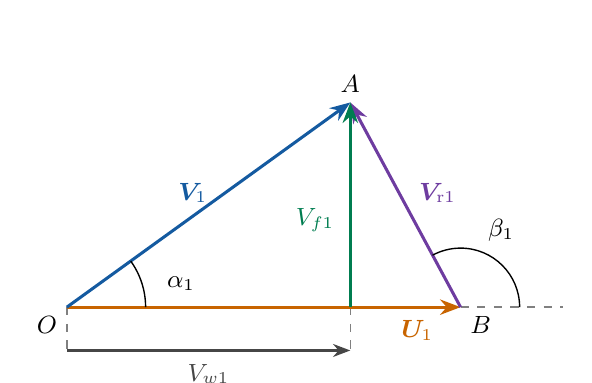
\begin{tikzpicture}[font=\small]
  \coordinate (O) at (0,0);
  \coordinate (B) at (5,0);
  \coordinate (P) at (3.6,0);
  \coordinate (A) at (3.6,2.6);
  % guides
  \draw[ref] (3.6,0)--(3.6,-0.55);
  \draw[ref] (0,0)--(0,-0.55);
  \draw[ref] (B)--(6.3,0);
  % vectors
  \draw[vU] (O)--(B);
  \draw[vV] (O)--(A);
  \draw[vR] (B)--(A);
  \draw[vF] (P)--(A);
  \draw[vW] (0,-0.55)--(3.6,-0.55);
  % labels
  \node[cV] at (1.6,1.45) {$\bm V_1$};
  \node[cR,right] at (4.35,1.45) {$\bm V_{\mathrm r1}$};
  \node[cF,left] at (3.52,1.1) {$V_{f1}$};
  \node[cW,below] at (1.8,-0.6) {$V_{w1}$};
  \node[cU,below] at (4.45,-0.05) {$\bm U_1$};
  \node[below left] at (O) {$O$};
  \node[below right] at (B) {$B$};
  \node[above] at (A) {$A$};
  % angles
  \draw[ang] (1.0,0) arc (0:35.8:1.0);
  \node at (1.45,0.3) {$\alpha_1$};
  \draw[ang] ([shift={(0:0.75)}]B) arc (0:118.3:0.75);
  \node at ([shift={(62:1.1)}]B) {$\beta_1$};
\end{tikzpicture}
\caption{Inlet velocity triangle for $V_{w1} < U_1$. Vector sum: $\bm V_1 = \bm U_1 + \bm V_{\mathrm r1}$, with $\bm V_{\mathrm r1}$ directed from $B$ (head of $\bm U_1$) to $A$ (head of $\bm V_1$). The angle $\alpha_1$ is measured from the positive tangential direction to $\bm V_1$; $\beta_1$ is measured from the positive tangential direction (dashed extension of $\bm U_1$) to $\bm V_{\mathrm r1}$ and is obtuse.}
\label{fig:inlet-a}
\end{figure}

\subsubsection{Case \texorpdfstring{$V_{w1} > U_1$}{Vw1 > U1}}

The tangential component $V_{w1}-U_1$ is positive; $\vvec{V}_{\vr 1}$ points forwards and $\beta_1 < 90^\circ$. The tangential component of the relative velocity is the dashed segment $BP$ in Figure~\ref{fig:inlet-b}.

\begin{figure}[h!]
\centering
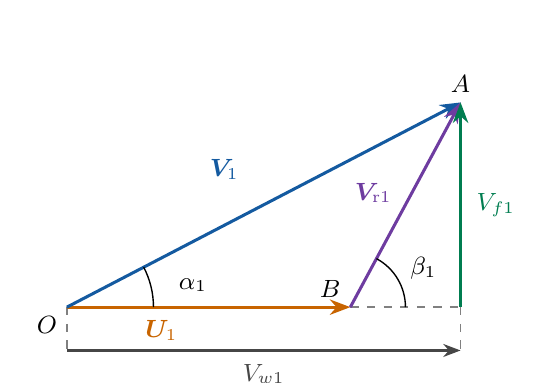
\begin{tikzpicture}[font=\small]
  \coordinate (O) at (0,0);
  \coordinate (B) at (3.6,0);
  \coordinate (P) at (5,0);
  \coordinate (A) at (5,2.6);
  \draw[ref] (B)--(P);
  \draw[ref] (P)--(5,-0.55);
  \draw[ref] (0,0)--(0,-0.55);
  \draw[vU] (O)--(B);
  \draw[vV] (O)--(A);
  \draw[vR] (B)--(A);
  \draw[vF] (P)--(A);
  \draw[vW] (0,-0.55)--(5,-0.55);
  \node[cV] at (2.0,1.75) {$\bm V_1$};
  \node[cR,left] at (4.25,1.45) {$\bm V_{\mathrm r1}$};
  \node[cF,right] at (5.08,1.3) {$V_{f1}$};
  \node[cW,below] at (2.5,-0.6) {$V_{w1}$};
  \node[cU,below] at (1.2,-0.05) {$\bm U_1$};
  \node[below left] at (O) {$O$};
  \node[above left] at (B) {$B$};
  \node[above] at (A) {$A$};
  \draw[ang] (1.1,0) arc (0:27.5:1.1);
  \node at (1.6,0.28) {$\alpha_1$};
  \draw[ang] ([shift={(0:0.7)}]B) arc (0:61.7:0.7);
  \node at ([shift={(28:1.05)}]B) {$\beta_1$};
\end{tikzpicture}
\caption{Inlet velocity triangle for $V_{w1} > U_1$. The vector $\bm V_{\mathrm r1}$ again runs from $B$ (head of $\bm U_1$) to $A$ (head of $\bm V_1$). Both $\alpha_1$ and $\beta_1$ are measured from the positive tangential direction and are acute.}
\label{fig:inlet-b}
\end{figure}

\subsection{Outlet velocity triangle and radial discharge}
\label{sec:outlet}

At the outlet,
\begin{equation}
  \vvec{V}_2 = \vvec{U}_2 + \vvec{V}_{\vr 2}, \qquad U_2 = \frac{\pi D_2 N}{60}.
  \label{eq:outlet-vec}
\end{equation}
For \emph{radial discharge} the absolute velocity leaves the runner without whirl:
\begin{equation}
  V_{w2} = 0, \qquad V_2 = V_{f2}, \qquad \alpha_2 = 90^\circ .
  \label{eq:radial}
\end{equation}
The relative velocity and its angle, with $\beta_2$ measured from the positive tangential direction, follow from the right-angled triangle of Figure~\ref{fig:outlet}:
\begin{equation}
  V_{\vr 2} = \sqrt{U_2^{2} + V_{f2}^{2}}, \qquad
  \beta_2 = 180^\circ - \arctan\frac{V_{f2}}{U_2}.
  \label{eq:outlet-rel}
\end{equation}
The acute angle between $\vvec{V}_{\vr 2}$ and the \emph{negative} tangential direction is $\arctan(V_{f2}/U_2) = 180^\circ-\beta_2$; this is the value commonly quoted as the outlet vane angle in texts that use the backward-tangent reference.

\begin{figure}[h!]
\centering
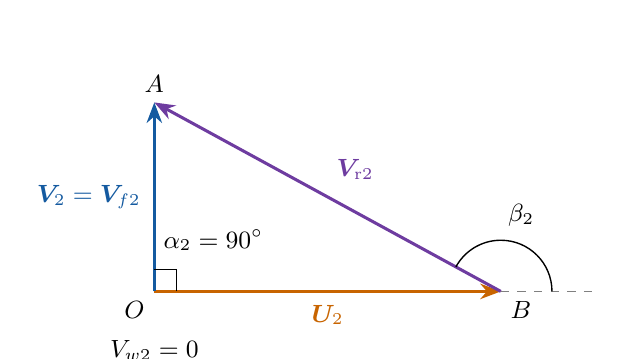
\begin{tikzpicture}[font=\small]
  \coordinate (O) at (0,0);
  \coordinate (B) at (4.4,0);
  \coordinate (A) at (0,2.4);
  \draw[ref] (B)--(5.6,0);
  \draw[vU] (O)--(B);
  \draw[vV] (O)--(A);
  \draw[vR] (B)--(A);
  \draw[ang] (0.28,0)--(0.28,0.28)--(0,0.28);
  \node[cV,left] at (-0.05,1.2) {$\bm V_2 = \bm V_{f2}$};
  \node[cR] at (2.55,1.55) {$\bm V_{\mathrm r2}$};
  \node[cU,below] at (2.2,-0.05) {$\bm U_2$};
  \node[below] at (0,-0.5) {$V_{w2}=0$};
  \node[below left] at (O) {$O$};
  \node[below right] at (B) {$B$};
  \node[above] at (A) {$A$};
  \draw[ang] ([shift={(0:0.65)}]B) arc (0:151.4:0.65);
  \node at ([shift={(75:1.0)}]B) {$\beta_2$};
  \node at (0.75,0.65) {$\alpha_2=90^\circ$};
\end{tikzpicture}
\caption{Outlet velocity triangle for radial discharge ($V_{w2}=0$). The absolute velocity $\bm V_2$ is perpendicular to $\bm U_2$; $\bm V_{\mathrm r2}$ runs from $B$ (head of $\bm U_2$) to $A$ (head of $\bm V_2$). The angle $\beta_2$ is measured from the positive tangential direction and is obtuse.}
\label{fig:outlet}
\end{figure}

Radial discharge does not imply $U_2 = 0$; it implies only that the absolute velocity at the runner exit has no tangential component.

\subsection{Construction procedure}
\label{sec:construction}

\begin{enumerate}[nosep]
  \item Draw $\vvec{U}$ along the positive tangential direction from a point $O$ to a point $B$.
  \item From $O$, draw $\vvec{V}$ with the specified whirl and flow components (or with the specified angle $\alpha$ and magnitude).
  \item Draw $\vvec{V}_\vr$ from $B$ to the head $A$ of $\vvec{V}$, in accordance with Eq.~\eqref{eq:vector-rel}.
  \item Evaluate the signed tangential difference $V_w - U$ to establish the direction of $\vvec{V}_\vr$.
  \item Mark each angle from its stated reference direction.
\end{enumerate}

%-------------------------------------------------- 4
\section{Work Done: the Euler Turbine Equation}
\label{sec:euler}

For a mass flow rate $\dot m$ passing through the runner, the change of angular momentum between inlet and outlet gives the torque on the runner,
\begin{equation}
  T = \dot m\,(r_1 V_{w1} - r_2 V_{w2}).
  \label{eq:torque}
\end{equation}
Multiplying by $\omega$ and using $U = \omega r$, the power transferred to the runner is
\begin{equation}
  P = T\omega = \dot m\,(U_1 V_{w1} - U_2 V_{w2}).
  \label{eq:power}
\end{equation}
The work done per unit mass of water is therefore
\begin{equation}
  w = U_1 V_{w1} - U_2 V_{w2} \qquad [\si{J/kg}],
  \label{eq:work-mass}
\end{equation}
and the work done per unit weight (the head extracted by the runner) is
\begin{equation}
  h_r = \frac{U_1 V_{w1} - U_2 V_{w2}}{g} \qquad [\si{m}].
  \label{eq:work-weight}
\end{equation}
For radial discharge, Eq.~\eqref{eq:radial} reduces Eqs.~\eqref{eq:work-mass} and~\eqref{eq:work-weight} to
\begin{equation}
  w = U_1 V_{w1}, \qquad h_r = \frac{U_1 V_{w1}}{g}.
  \label{eq:work-radial}
\end{equation}
\emph{Dimensional check:} $UV_w$ has units $\si{m^2/s^2} = \si{J/kg}$; division by $g$ gives metres.

%-------------------------------------------------- 5
\section{Efficiencies}
\label{sec:efficiencies}

Each efficiency refers to a particular energy boundary and must be applied accordingly.

\subsection{Hydraulic efficiency}

The hydraulic efficiency is the ratio of the head extracted by the runner to the net head $H$:
\begin{equation}
  \eta_H = \frac{h_r}{H} = \frac{U_1 V_{w1} - U_2 V_{w2}}{gH},
  \label{eq:etaH}
\end{equation}
which for radial discharge becomes
\begin{equation}
  \eta_H = \frac{U_1 V_{w1}}{gH}.
  \label{eq:etaH-radial}
\end{equation}

\subsection{Volumetric efficiency}

Part of the supplied discharge $Q_1$ may leak past the runner. If $Q_2 = Q_1 - \Delta Q$ is the discharge that actually passes through the runner passages,
\begin{equation}
  \eta_{\mathrm{vol}} = \frac{Q_2}{Q_1} = \frac{Q_1 - \Delta Q}{Q_1}.
  \label{eq:etavol}
\end{equation}

\subsection{Mechanical efficiency}

Mechanical losses in bearings, seals and other rotating components reduce the shaft power relative to the power developed by the runner:
\begin{equation}
  \eta_{\mathrm{mech}} = \frac{P_{\mathrm{shaft}}}{P_{\mathrm{runner}}}.
  \label{eq:etamech}
\end{equation}

\subsection{Overall efficiency}

The overall efficiency relates the shaft power to the power supplied by the water,
\begin{equation}
  \eta_o = \frac{P_{\mathrm{shaft}}}{\rho g Q_1 H}.
  \label{eq:etao}
\end{equation}
The power developed by the runner follows from Eq.~\eqref{eq:power} with $\dot m = \rho Q_2$, and from Eqs.~\eqref{eq:etaH} and~\eqref{eq:etavol},
\begin{equation}
  P_{\mathrm{runner}} = \rho Q_2\,(U_1 V_{w1} - U_2 V_{w2}) = \eta_H\,\rho g Q_2 H = \eta_H\,\eta_{\mathrm{vol}}\,\rho g Q_1 H.
  \label{eq:Prunner}
\end{equation}
Substituting Eq.~\eqref{eq:Prunner} in Eq.~\eqref{eq:etamech} and comparing with Eq.~\eqref{eq:etao} gives
\begin{equation}
  \eta_o = \eta_H\,\eta_{\mathrm{vol}}\,\eta_{\mathrm{mech}}.
  \label{eq:etaproduct}
\end{equation}

\subsection{Draft-tube efficiency}

The draft-tube efficiency measures the effectiveness of pressure recovery downstream of the runner:
\begin{equation}
  \eta_d = \frac{\dfrac{V_3^{2} - V_4^{2}}{2g} - h_f}{\dfrac{V_3^{2}}{2g}},
  \label{eq:etad}
\end{equation}
where $V_3$ and $V_4$ are the velocities at the draft-tube inlet and outlet respectively and $h_f$ is the head loss in the draft tube. The inlet velocity is normally taken as the runner-exit velocity, $V_3 = V_2$. The draft-tube efficiency is not a factor in the product~\eqref{eq:etaproduct}.

\subsection{Energy-balance form of the hydraulic efficiency}

If the only loss associated with the runner and its surroundings is the kinetic energy discharged with the water at the turbine outlet (velocity $V_e$), the hydraulic efficiency may also be written
\begin{equation}
  \eta_H = \frac{H - \dfrac{V_e^{2}}{2g}}{H}.
  \label{eq:etaH-balance}
\end{equation}
This expression is equivalent to Eq.~\eqref{eq:etaH} only under the stated assumption of no other hydraulic losses. Where whirl components are specified or required, Eq.~\eqref{eq:etaH} is the appropriate form.

%-------------------------------------------------- 6
\section{Working Proportions and Discharge}
\label{sec:proportions}

Two dimensionless ratios are used in the preliminary design of Francis runners:
\begin{equation}
  \phi = \frac{U_1}{\sqrt{2gH}}, \qquad \psi = \frac{V_{f1}}{\sqrt{2gH}},
  \label{eq:ratios}
\end{equation}
the \emph{speed ratio} $\phi$ (typically $0.6$--$0.9$) and the \emph{flow ratio} $\psi$ (typically $0.15$--$0.30$).

If $n$ vanes of thickness $t$ obstruct the inlet circumference $\pi D_1$, the effective inlet flow area is
\begin{equation}
  A_{f1} = (\pi D_1 - n t)\,B_1 = C\,\pi D_1 B_1, \qquad C = 1 - \frac{n t}{\pi D_1},
  \label{eq:area}
\end{equation}
where $C$ is the contraction factor. The discharge passing through the runner is then
\begin{equation}
  Q_2 = C\,\pi D_1 B_1 V_{f1}.
  \label{eq:Qrunner}
\end{equation}
The following simplified proportions are commonly adopted in preliminary design:
\begin{equation}
  D_1 = 2D_2, \qquad V_{f1} = V_{f2}, \qquad B_2 = 2B_1 .
  \label{eq:proportions}
\end{equation}
These are design assumptions, not general identities. Under Eq.~\eqref{eq:proportions}, and with the same contraction factor at inlet and outlet, continuity $C\pi D_1 B_1 V_{f1} = C\pi D_2 B_2 V_{f2}$ is satisfied identically.

%-------------------------------------------------- 7
\section{Worked Numerical Example}
\label{sec:example}

\subsection{General solution procedure}

\begin{enumerate}[nosep]
  \item List the given data in SI units and identify the required quantities.
  \item Evaluate $\sqrt{2gH}$ and obtain $U_1 = \phi\sqrt{2gH}$ and $V_{f1} = \psi\sqrt{2gH}$ from Eq.~\eqref{eq:ratios}.
  \item Obtain the overall efficiency from Eq.~\eqref{eq:etaproduct} and the discharge from Eq.~\eqref{eq:etao}.
  \item Obtain the runner diameters from Eq.~\eqref{eq:U} and the proportions~\eqref{eq:proportions}.
  \item With radial discharge, obtain $V_{w1}$ from Eq.~\eqref{eq:etaH-radial}.
  \item Compute the velocity triangles from Eqs.~\eqref{eq:alpha1}--\eqref{eq:beta1} and~\eqref{eq:outlet-rel}.
  \item Obtain the blade width from Eq.~\eqref{eq:Qrunner}, and verify the result by an independent power check.
\end{enumerate}

\subsection{Problem statement}

A Francis turbine operates under a net head of $H = \SI{60}{m}$ and rotates at $N = \SI{300}{rpm}$. It delivers a shaft power $P_{\mathrm{shaft}} = \SI{3.5}{MW}$. The hydraulic, volumetric and mechanical efficiencies are $\eta_H = 0.90$, $\eta_{\mathrm{vol}} = 0.98$ and $\eta_{\mathrm{mech}} = 0.96$. The speed ratio is $\phi = 0.70$, the flow ratio is $\psi = 0.16$, and the contraction factor due to vane thickness is $C = 0.95$. Discharge from the runner is radial. The proportions of Eq.~\eqref{eq:proportions} apply. Take $\rho = \SI{1000}{kg/m^3}$ and $g = \SI{9.81}{m/s^2}$.

Determine: (a)~the overall efficiency and the discharge; (b)~the runner diameters and the peripheral velocities; (c)~the inlet velocity triangle (all velocities and angles); (d)~the outlet velocity triangle; (e)~the blade widths at inlet and outlet; and (f)~verify the shaft power.

\subsection{Solution}

\paragraph{Step 1: Reference velocity, peripheral and flow velocities at inlet.}
\begin{align}
  \sqrt{2gH} &= \sqrt{2(9.81)(60)} = \SI{34.31}{m/s}, \label{eq:ex-ref}\\
  U_1 &= \phi\sqrt{2gH} = 0.70(34.31) = \SI{24.02}{m/s}, \label{eq:ex-U1}\\
  V_{f1} &= \psi\sqrt{2gH} = 0.16(34.31) = \SI{5.49}{m/s}. \label{eq:ex-Vf1}
\end{align}

\paragraph{Step 2: Overall efficiency and discharge.} From Eq.~\eqref{eq:etaproduct},
\begin{equation}
  \eta_o = \eta_H\,\eta_{\mathrm{vol}}\,\eta_{\mathrm{mech}} = 0.90(0.98)(0.96) = 0.8467.
  \label{eq:ex-eta}
\end{equation}
From Eq.~\eqref{eq:etao}, the supplied discharge and the discharge through the runner are
\begin{align}
  Q_1 &= \frac{P_{\mathrm{shaft}}}{\eta_o\,\rho g H} = \frac{3.5\times10^{6}}{0.8467(1000)(9.81)(60)} = \SI{7.023}{m^3/s}, \label{eq:ex-Q1}\\
  Q_2 &= \eta_{\mathrm{vol}}\,Q_1 = 0.98(7.023) = \SI{6.882}{m^3/s}. \label{eq:ex-Q2}
\end{align}

\paragraph{Step 3: Runner diameters and peripheral velocities.} From Eq.~\eqref{eq:U} and Eq.~\eqref{eq:proportions},
\begin{align}
  D_1 &= \frac{60\,U_1}{\pi N} = \frac{60(24.02)}{\pi(300)} = \SI{1.529}{m}, \label{eq:ex-D1}\\
  D_2 &= \frac{D_1}{2} = \SI{0.7645}{m}, \label{eq:ex-D2}\\
  U_2 &= \frac{\pi D_2 N}{60} = \frac{\pi(0.7645)(300)}{60} = \SI{12.01}{m/s}. \label{eq:ex-U2}
\end{align}

\paragraph{Step 4: Inlet velocity triangle.} With $V_{w2}=0$, Eq.~\eqref{eq:etaH-radial} gives
\begin{equation}
  V_{w1} = \frac{\eta_H\,gH}{U_1} = \frac{0.90(9.81)(60)}{24.02} = \SI{22.06}{m/s}.
  \label{eq:ex-Vw1}
\end{equation}
Since $V_{w1} < U_1$, the inlet triangle is of the type shown in Figure~\ref{fig:inlet-a}. From Eqs.~\eqref{eq:V1}, \eqref{eq:alpha1}, \eqref{eq:Vr1} and~\eqref{eq:beta1},
\begin{align}
  V_1 &= \sqrt{22.06^{2} + 5.49^{2}} = \SI{22.73}{m/s}, \label{eq:ex-V1}\\
  \alpha_1 &= \arctan\frac{5.49}{22.06} = \SI{13.98}{\degree}, \label{eq:ex-alpha1}\\
  V_{w1} - U_1 &= 22.06 - 24.02 = \SI{-1.96}{m/s}, \label{eq:ex-diff}\\
  V_{\vr 1} &= \sqrt{(-1.96)^{2} + 5.49^{2}} = \SI{5.83}{m/s}, \label{eq:ex-Vr1}\\
  \beta_1 &= \operatorname{atan2}(5.49,\,-1.96) = 180^\circ - \arctan\frac{5.49}{1.96} = \SI{109.65}{\degree}. \label{eq:ex-beta1}
\end{align}
The angle $\beta_1$ is obtuse because $V_{w1}-U_1<0$ (reference: positive tangential direction). Its supplement, $\SI{70.35}{\degree}$, is the acute angle with the negative tangential direction.

\paragraph{Step 5: Outlet velocity triangle.} For radial discharge, Eq.~\eqref{eq:radial} and $V_{f2} = V_{f1}$ give
\begin{equation}
  V_{w2} = 0, \qquad V_2 = V_{f2} = \SI{5.49}{m/s}, \qquad \alpha_2 = 90^\circ,
  \label{eq:ex-V2}
\end{equation}
and from Eq.~\eqref{eq:outlet-rel},
\begin{align}
  V_{\vr 2} &= \sqrt{12.01^{2} + 5.49^{2}} = \SI{13.20}{m/s}, \label{eq:ex-Vr2}\\
  \beta_2 &= 180^\circ - \arctan\frac{5.49}{12.01} = 180^\circ - 24.57^\circ = \SI{155.43}{\degree}. \label{eq:ex-beta2}
\end{align}
Both triangles are drawn to a common scale in Figure~\ref{fig:example}.

\paragraph{Step 6: Blade widths.} From Eq.~\eqref{eq:Qrunner},
\begin{equation}
  B_1 = \frac{Q_2}{C\pi D_1 V_{f1}} = \frac{6.882}{0.95\,\pi\,(1.529)(5.49)} = \SI{0.2747}{m},
  \label{eq:ex-B1}
\end{equation}
and from Eq.~\eqref{eq:proportions},
\begin{equation}
  B_2 = 2B_1 = \SI{0.5495}{m}.
  \label{eq:ex-B2}
\end{equation}
Continuity at the outlet is confirmed by
\begin{equation}
  C\pi D_2 B_2 V_{f2} = 0.95\,\pi\,(0.7645)(0.5495)(5.49) = \SI{6.88}{m^3/s} = Q_2.
  \label{eq:ex-cont}
\end{equation}

\paragraph{Step 7: Verification of the shaft power.} The runner power from Eq.~\eqref{eq:Prunner}, and the shaft power from Eq.~\eqref{eq:etamech}, are
\begin{align}
  P_{\mathrm{runner}} &= \rho Q_2\,U_1 V_{w1} = 1000(6.882)(24.02)(22.06) = \SI{3.646}{MW}, \label{eq:ex-Pr}\\
  P_{\mathrm{shaft}} &= \eta_{\mathrm{mech}}\,P_{\mathrm{runner}} = 0.96(3.646) = \SI{3.50}{MW}. \label{eq:ex-Ps}
\end{align}
This reproduces the specified shaft power. As a further check, the head extracted by the runner from Eq.~\eqref{eq:work-radial} is $h_r = U_1 V_{w1}/g = 24.02(22.06)/9.81 = \SI{54.0}{m}$, so that $\eta_H = 54.0/60 = 0.90$, in agreement with the given value. The ratios $\phi = 0.70$ and $\psi = 0.16$ lie within the ranges stated in Section~\ref{sec:proportions}.

\begin{figure}[h!]
\centering
\def\sc{0.27}
\begin{tikzpicture}[font=\small]
  % ---- inlet (origin at left), scale 0.27 cm per m/s
  \begin{scope}
    \coordinate (O1) at (0,0);
    \coordinate (B1) at ({\sc*24.02},0);
    \coordinate (P1) at ({\sc*22.06},0);
    \coordinate (A1) at ({\sc*22.06},{\sc*5.49});
    \draw[ref] (B1)--++(1.2,0);
    \draw[vU] (O1)--(B1);
    \draw[vV] (O1)--(A1);
    \draw[vR] (B1)--(A1);
    \draw[vF] (P1)--(A1);
    \node[cV] at (3.0,1.05) {$\bm V_1$};
    \node[cR] at ([shift={(75:1.15)}]B1) {$\bm V_{\mathrm r1}$};
    \node[cF,left] at ({\sc*22.0},0.75) {$V_{f1}$};
    \node[cU,below] at (3.3,-0.05) {$\bm U_1$};
    \node[below left] at (O1) {$O$};
    \node[below right] at (B1) {$B$};
    \node[above] at (A1) {$A$};
    \draw[ang] (1.5,0) arc (0:13.98:1.5);
    \node at (1.85,0.22) {$\alpha_1$};
    \draw[ang] ([shift={(0:0.6)}]B1) arc (0:109.65:0.6);
    \node at ([shift={(22:0.95)}]B1) {$\beta_1$};
    \node[align=center,anchor=north] at (3.3,-0.85) {(a) Inlet\\[-1pt]$V_{w1}=\SI{22.06}{m/s}$, $U_1=\SI{24.02}{m/s}$\\[-1pt]$V_{f1}=\SI{5.49}{m/s}$};
  \end{scope}
  % ---- outlet
  \begin{scope}[xshift=9.2cm]
    \coordinate (O2) at (0,0);
    \coordinate (B2) at ({\sc*12.01},0);
    \coordinate (A2) at (0,{\sc*5.49});
    \draw[ref] (B2)--++(0.9,0);
    \draw[vU] (O2)--(B2);
    \draw[vV] (O2)--(A2);
    \draw[vR] (B2)--(A2);
    \draw[ang] (0.2,0)--(0.2,0.2)--(0,0.2);
    \node[cV,left] at (-0.05,0.75) {$\bm V_2$};
    \node[cR] at (1.9,1.0) {$\bm V_{\mathrm r2}$};
    \node[cU,below] at (1.6,-0.05) {$\bm U_2$};
    \node[below left] at (O2) {$O$};
    \node[below right] at (B2) {$B$};
    \node[above] at (A2) {$A$};
    \draw[ang] ([shift={(0:0.55)}]B2) arc (0:155.43:0.55);
    \node at ([shift={(72:0.9)}]B2) {$\beta_2$};
    \node[align=center,anchor=north] at (1.6,-0.85) {(b) Outlet\\[-1pt]$V_2=V_{f2}=\SI{5.49}{m/s}$, $U_2=\SI{12.01}{m/s}$\\[-1pt]$V_{w2}=0$};
  \end{scope}
\end{tikzpicture}
\caption{Velocity triangles of the worked example, drawn to a common scale ($\SI{1}{cm} \approx \SI{3.7}{m/s}$). (a) Inlet: $\alpha_1 = \SI{13.98}{\degree}$, $\beta_1 = \SI{109.65}{\degree}$. (b) Outlet: $\alpha_2 = 90^\circ$, $\beta_2 = \SI{155.43}{\degree}$. Angles are measured from the positive tangential direction; $\bm V_{\mathrm r}$ runs from the head of $\bm U$ to the head of $\bm V$ in both triangles.}
\label{fig:example}
\end{figure}

\subsection{Summary of results}

\begin{table}[h!]
\centering
\begin{tabular}{@{}lcc@{}}
\toprule
Quantity & Inlet (1) & Outlet (2)\\
\midrule
Runner diameter $D$ (\si{m}) & 1.529 & 0.7645\\
Blade width $B$ (\si{m}) & 0.2747 & 0.5495\\
Peripheral velocity $U$ (\si{m/s}) & 24.02 & 12.01\\
Whirl velocity $V_w$ (\si{m/s}) & 22.06 & 0\\
Flow velocity $V_f$ (\si{m/s}) & 5.49 & 5.49\\
Absolute velocity $V$ (\si{m/s}) & 22.73 & 5.49\\
Relative velocity $V_\vr$ (\si{m/s}) & 5.83 & 13.20\\
Absolute-flow angle $\alpha$ (\si{\degree}) & 13.98 & 90\\
Relative-flow angle $\beta$ (\si{\degree}) & 109.65 & 155.43\\
\midrule
\multicolumn{3}{@{}l}{$\eta_o = 0.8467$, \quad $Q_1 = \SI{7.023}{m^3/s}$, \quad $Q_2 = \SI{6.882}{m^3/s}$, \quad $P_{\mathrm{runner}} = \SI{3.646}{MW}$}\\
\bottomrule
\end{tabular}
\caption{Results of the numerical example. Angles are referred to the positive tangential direction.}
\label{tab:results}
\end{table}

%-------------------------------------------------- 8
\section{Summary of Formulae}
\label{sec:summary}

\begin{center}
\begin{tabular}{@{}p{5.2cm}p{6.6cm}c@{}}
\toprule
Quantity & Expression & Eq.\\
\midrule
Vector relation & $\vvec{V} = \vvec{U} + \vvec{V}_\vr$ & \eqref{eq:vector}\\
Peripheral velocity & $U = \pi D N/60$ & \eqref{eq:U}\\
Absolute velocity magnitude & $V = \sqrt{V_w^2 + V_f^2}$ & \eqref{eq:Vmag}\\
Inlet absolute-flow angle & $\tan\alpha_1 = V_{f1}/V_{w1}$ & \eqref{eq:alpha1}\\
Inlet relative-flow angle & $\tan\beta_1 = V_{f1}/(V_{w1}-U_1)$ (signed) & \eqref{eq:beta1}\\
Radial outlet & $V_{w2}=0,\ V_2=V_{f2},\ \alpha_2=90^\circ$ & \eqref{eq:radial}\\
Outlet relative velocity and angle & $V_{\vr 2}=\sqrt{U_2^2+V_{f2}^2}$, $\beta_2=180^\circ-\arctan(V_{f2}/U_2)$ & \eqref{eq:outlet-rel}\\
Work per unit mass & $w = U_1V_{w1}-U_2V_{w2}$ & \eqref{eq:work-mass}\\
Work per unit weight & $h_r = (U_1V_{w1}-U_2V_{w2})/g$ & \eqref{eq:work-weight}\\
Hydraulic efficiency & $\eta_H = (U_1V_{w1}-U_2V_{w2})/(gH)$ & \eqref{eq:etaH}\\
Volumetric efficiency & $\eta_{\mathrm{vol}} = Q_2/Q_1$ & \eqref{eq:etavol}\\
Mechanical efficiency & $\eta_{\mathrm{mech}} = P_{\mathrm{shaft}}/P_{\mathrm{runner}}$ & \eqref{eq:etamech}\\
Overall efficiency & $\eta_o = P_{\mathrm{shaft}}/(\rho gQ_1H)$ & \eqref{eq:etao}\\
Efficiency product & $\eta_o = \eta_H\eta_{\mathrm{vol}}\eta_{\mathrm{mech}}$ & \eqref{eq:etaproduct}\\
Speed and flow ratios & $\phi = U_1/\sqrt{2gH},\ \psi = V_{f1}/\sqrt{2gH}$ & \eqref{eq:ratios}\\
Runner discharge & $Q_2 = C\pi D_1B_1V_{f1}$ & \eqref{eq:Qrunner}\\
\bottomrule
\end{tabular}
\captionof{table}{Summary of principal formulae.}\label{tab:formulae}
\end{center}

%-------------------------------------------------- 9
\section{Common Errors}
\label{sec:errors}

\begin{itemize}[nosep]
  \item A velocity triangle rotated or reflected on the page represents the same physical case; vector directions and arrowheads, not page orientation, carry the information.
  \item The relation $\vvec{V}_\vr = \vvec{V} - \vvec{U}$, Eq.~\eqref{eq:vector-rel}, fixes the direction of the relative velocity; the magnitude relation~\eqref{eq:Vmag} must not be substituted for it.
  \item An angle is incomplete unless its reference direction is stated (Section~\ref{sec:conventions}).
  \item The sign of $V_{w1}-U_1$ must be retained in Eq.~\eqref{eq:beta1}; discarding it changes an obtuse $\beta_1$ into its supplement.
  \item Radial discharge means $V_{w2}=0$, not $U_2=0$.
  \item Work per unit mass is expressed in \si{J/kg}; work per unit weight is expressed in metres of head.
  \item The overall efficiency $\eta_o$ includes volumetric and mechanical effects and is not equal to $\eta_H$.
  \item The draft-tube efficiency, Eq.~\eqref{eq:etad}, is distinct from the product in Eq.~\eqref{eq:etaproduct}.
  \item The discharge used in the runner-area relation, Eq.~\eqref{eq:Qrunner}, is the discharge through the runner, $Q_2 = \eta_{\mathrm{vol}}Q_1$, not the supplied discharge $Q_1$.
\end{itemize}

\end{document}
